\documentclass[12pt,addpoints]{exam}
\usepackage[utf8]{inputenc}
\usepackage{lastpage}
\usepackage{amsmath}
\usepackage{amsfonts}
\usepackage{amssymb}
\usepackage{enumerate}
\usepackage{mdframed}
\usepackage{array}
\usepackage{graphics}
\usepackage{graphicx}
\usepackage{listings}
\usepackage{tikz}
\usetikzlibrary{arrows}
\usepackage{algpseudocode}

% Paramètres globaux
\bonuspointpoints{point \emph{bonus}}{points \emph{boni}}
\parindent 0cm
\hqword{Question}
\hpword{Sur}
\hsword{Note}
\htword{Total}

% Réponses
%\printanswers

% En-tête et pieds de page
\headrule
\cfoot{\thepage /\pageref{LastPage}}
\lhead{CS Games --- Informatique théorique}
\rhead{Hiver 2016}
\newcommand{\headrulewidth}{0.4pt}
\newcommand{\footrulewidth}{0.4pt}

% Raccourcis
\newcommand{\bigo}{\mathcal{O}}
\newcommand{\N}{\mathbb{N}}
\newcommand{\R}{\mathbb{R}}

% Algorithmes
\algrenewcommand\algorithmicwhile{\textbf{tant que}}
\algrenewcommand\algorithmicfunction{\textbf{fonction}}
\algrenewcommand\algorithmicend{\textbf{fin}}
\algrenewcommand\algorithmicdo{\textbf{faire}}
\algrenewcommand\algorithmicfor{\textbf{pour}}
\algrenewcommand\algorithmicif{\textbf{si}}
\algrenewcommand\algorithmicelse{\textbf{sinon}}
\algrenewcommand\algorithmicthen{\textbf{alors}}
\algrenewcommand\algorithmicreturn{\textbf{retourner}}
\algrenewcommand\algorithmicrepeat{\textbf{faire}}
\algrenewcommand\algorithmicuntil{\textbf{tant que}}
\newcommand{\enteteproc}[2]{\vskip\baselineskip \hspace*{\fill} \algorithmicprocedure~\Call{#1}{#2} \hspace*{\fill} \vskip\baselineskip}
\newcommand{\entetefunc}[3]{\vskip\baselineskip \hspace*{\fill} \algorithmicfunction~\Call{#1}{#2} : #3 \hspace*{\fill} \vskip\baselineskip}

\begin{document}
	
\allowdisplaybreaks

\thispagestyle{empty}
~\vfill
\ifprintanswers
  \vskip 1.2cm
  \centerline{\Large\textbf{Solution de l'épreuve}}
  \vskip 0.5cm
\else
  \vskip 1.2cm
  \centerline{\Large\textbf{Épreuve d'informatique théorique}}
  \vskip 1.2cm
\fi
\hrule \vskip \baselineskip
Cette épreuve contient 20 questions réparties en 4 thèmes de 5 questions chacun~:
\begin{enumerate}
  \item La combinatoire;
  \item La théorie des graphes;
  \item La théorie des jeux;
  \item Les probabilités.
\end{enumerate}
La pondération est la même pour chacune des questions. Bonne chance !
\vskip \baselineskip \hrule
\vfill~
\newpage

\begin{questions}

% Combinatoire
\uplevel{Les questions suivantes portent sur la \textbf{combinatoire}, c'est-à-dire la théorie qui consiste à compter ou énumérer des objets.}

% Compter des mots
\question
On dit d'une chaîne binaire $w$ qu'elle \emph{évite} un motif $u$ si elle ne s'écrit pas sous la forme $w = xuy$, où $x$ et $y$ sont des mots quelconques (possiblement vides).
\begin{parts}
  \part Pour tout entier $n \geq 0$, soit $A(n)$ le nombre de chaînes binaires de longueur $n$ qui évitent le motif $0$. Donnez la valeur de $A(n)$ pour tout $n$.
  \part De la même façon, soit $B(n)$ le nombre de chaînes binaires de longueur $n$ qui évitent le motif $00$. Donnez la valeur de $B(n)$ pour toute valeur de $n$.
  \part Même question, mais avec $C(n)$ le nombre de chaînes binaires qui évitent le motif $000$.
\end{parts}

% Arbres binaires
\question
Un \emph{arbre binaire} est une arborescence dont chaque sommet a au plus $2$ enfants. Pour tout entier $n \geq 0$, soit $A(n)$ le nombre d'arbres de $n$ noeuds.
\begin{parts}
  \part Montrez que les premières valeurs de $A(n)$ sont bien celles illustrées dans le tableau ci-bas~:
  \begin{center} \begin{tabular}{c|ccccc}
    $n$    & 0 & 1 & 2 & 3 & 4 \\
    \hline
    $A(n)$ & 1 & 1 & 2 & 5 & 14 \\
  \end{tabular} \end{center}
  \part Il est bien connu que $A(n)$ vérifie les équations suivantes~:
  \begin{eqnarray*}
    A(0) & = & 1, \\
    A(n) & = & \sum_{i=0}^{n-1} A(i)A(n-i-1).
  \end{eqnarray*}
  Justifiez ces deux équations. \emph{Indice~:} Réfléchissez à la construction récursive des arbres binaires.
\end{parts}

% Numéros de téléphone
\question
TODO: Numéros de téléphone

% Chemins dans une grille
\question
Considérez une grille de $r$ rangées et $c$ colonnes (voir Figure~\ref{F:grille}). Dans cette question, on s'intéresse à compter le nombre de chemins à partir du point $(0,0)$ jusqu'au point $(c,r)$ n'utilisant que des déplacements vers la droite (identifiés par la lettre $d$) et vers le haut (identifiés par $h$). Donnez une formule qui compte le nombre de chemins distincts de $(0,0)$ vers $(c,r)$, pour toutes valeurs $r,c \geq 1$.

% 
\question
TODO

% Graphes
\uplevel{Les questions suivantes portent sur la \textbf{théorie des graphes}.
Un \emph{graphe simple} est un couple $G = (V,E)$ où $V$ est son ensemble de \emph{sommets} et $E \subseteq \mathcal{P}_2(V)$ est son ensemble d'\emph{arêtes}, où $\mathcal{P}_2(V)$ dénote l'ensemble des paires d'éléments distincts de $V$. Par exemple, le graphe $G = (V,E)$ défini par les ensembles
$$V = \{a,b,c,d\} \quad \text{et} \quad E = \{\{a,b\}, \{a,c\}, \{b,c\}, \{c,d\}\}$$
est représenté à la figure \ref{F:graphe}. À noter que dans un graphe simple, il n'y a pas d'arête multiple ni de boucle (une arête d'un sommet vers lui-même).}

% Familles de graphes
\question
Certaines familles de graphes simples sont souvent utilisées. En voici quelques-unes (voir figure~\ref{F:familles})~:
\begin{enumerate}[(i)]
  \item Pour tout entier $n \geq 1$, le graphe \emph{complet} de $n$ sommets $K_n$;
  \item Pour tout entier $n \geq 3$, le \emph{cycle} de $n$ sommets $C_n$;
  \item Pour tout entier $n \geq 3$, la \emph{roue} de $n + 1$ sommets $W_n$;
  \item Pour tout entier $n \geq 1$, l'\emph{hypercube} de dimension $n$ est noté $H_n$;
  \item Pour toute paire d'entiers $m,n \geq 1$, le graphe \emph{biparti complet} $K_{m,n}$;
\end{enumerate}
Pour toutes valeurs $n$ et $m$ bien définies, donnez le nombre d'arêtes des graphes suivants~:
\begin{parts}
  \part $K_n$;
  \part $C_n$;
  \part $W_n$;
  \part $H_n$;
  \part $K_{m,n}$.
\end{parts}

% Transversaux d'arêtes
\question
Soit $G = (V,E)$ un graphe simple. On dit d'un ensemble de sommets $U \subseteq V$ qu'il est un \emph{transversal d'arêtes} si chaque arête de $G$ a au moins une de ses extrémités dans $U$, c'est-à-dire que pour toute arête $\{u,v\} \in E$, on a $u \in U$ ou $v \in U$. Par exemple, dans le graphe de la figure \ref{F:graphe}, l'ensemble $\{a,c\}$ est un transversal d'arêtes. Un transversal d'arête $U$ est dit \emph{minimum} pour $G$ s'il n'existe aucun transversal d'arêtes $U'$ de plus petite cardinalité, c'est-à-dire tel que $|U'| < |U|$.

Pour toutes valeurs de $n$ et $m$ bien définies, donnez la taille d'un transversal d'arêtes minimum des graphes suivants~:
\begin{parts}
  \part $K_n$;
  \part $C_n$;
  \part $W_n$;
  \part $h_n$;
  \part $K_{m,n}$.
\end{parts}

% Problème HAMD
\question
On dit d'un graphe $G$ qu'il est \emph{hamiltonien} s'il admet au moins un cycle passant par chaque sommet \textbf{exactement} une fois.

Soit HAMD le problème de \emph{décider} si un graphe simple $G$ est hamiltonien ou non et soit HAM le problème de \emph{trouver} un cycle hamiltonien dans un graphe $G$ (on retourne la valeur \emph{rien} si un tel cycle n'existe pas). Autrement dit, on considère les deux fonctions suivantes~:
\begin{itemize}
  \item \Call{EstHamiltonien}{$G$ : graphe} : booléen;
  \item \Call{CycleHamiltonien}{$G$ : graphe} : cycle ou \emph{rien}.
\end{itemize}
Montrez que les deux problèmes sont de même difficulté à complexité polynomiale près. En d'autres termes, si $\textsc{EstHamiltonien}$ utilise un temps constant, alors on peut implémenter $\textsc{CycleHamiltonien}$ de telle sorte qu'elle utilise un temps polynomial (et vice-versa). \emph{Remarque~:} Vous devez écrire du pseudocode implémentant chacune des deux fonctions par rapport à l'autre.
\begin{solution}
Supposons d'abord que \textsc{CycleHamiltonien} utilise un temps constant. Alors la fonction
\begin{algorithmic}[1]
  \Function{EstHamiltonien}{$G$ : graphe} : booléen
    \State \Return \Call{CycleHamiltonien}{$G$}~$\neq$~rien
  \EndFunction
\end{algorithmic}
a également une complexité constante.

Réciproquement, supposons que \textsc{EstHamiltonien} utilise un temps constant et considérons la fonction suivante~:
\begin{algorithmic}[1]
  \Function{CycleHamiltonien}{$G = (V,E)$ : graphe} : cycle ou rien
    \If{$\neg \Call{EstHamiltonien}{G}$}
      \State \Return rien
    \Else
      \While{il existe $v \in V$ tel que $\deg(v) > 2$}
        \State Soit $v$ un sommet de degré au moins $3$
        \For{$u \in G.\Call{Voisins}{v}$}
          \State Soit $H$ le graphe obtenu de $G$ en supprimant $\{u,v\}$
          \If{$\Call{EstHamiltonien}{H}$}
            \State $G \leftarrow H$
          \EndIf
        \EndFor
      \EndWhile
      \State \Return l'unique cycle de $G$
    \EndIf
  \EndFunction
\end{algorithmic}
Sa complexité est de $\bigo(m(m + n)) = \bigo(m^2)$ qui est bien polynomiale.
\end{solution}

% Coloriages
\question\label{Q:kparti}
Étant donnés un graphe non orienté $G = (V,E)$ et un entier positif $k$, on dit d'une fonction $c : V \rightarrow \{1,2,\ldots,k\}$ qu'elle est un \emph{$k$-coloriage} de $G$ si pour toute arête $\{u,v\} \in E$, on a $c(u) \neq c(v)$, c'est-à-dire que deux sommets adjacents ont une couleur différente. Si $G$ peut être colorié à l'aide de $k$ couleurs, alors on dit qu'il est $k$-coloriable.

D'autre part, on dit que $G$ est $k$-parti s'il existe des ensembles $V_1, V_2, \ldots, V_k$ tels que
\begin{enumerate}
  \item $V_1 \cup V_2 \cup \cdots \cup V_k = V$,
  \item $V_i \cap V_j = \emptyset$ et
  \item Pour tout arête $\{u,v\}$, si $u \in V_i$ et $v \in V_j$, alors $i = j$.
\end{enumerate}
Autrement dit, on peut partitionner l'ensemble de sommets $V$ en $k$ morceaux de sorte que les arêtes reliant deux sommets dans un même morceau sont interdites.

Montrez que tout graphe $k$-parti est $k$-coloriable.

% P-équivalence coloriages
\question
Soit $k$-COLORD le problème de \emph{décider} si un graphe non orienté $G$ est $k$-coloriable et $k$-COLOR le problème de \emph{trouver} un $k$-coloriage de $G$. Montrez que les problèmes $k$-COLORD et $k$-COLOR sont de même difficulté à complexité polynomiale près. \emph{Indice~:} La question~\ref{Q:kparti} devrait vous être utile.

% Jeux
\uplevel{Les questions suivantes portent sur la \textbf{théorie des jeux}.}

% Jeu de Nim
\question
Cette question porte sur le célèbre \emph{jeu de Nim}, aussi appelé \emph{jeu des allumettes}. Il s'agit d'un jeu à deux joueurs, appelés joueur A et joueur B, qui, à tour de rôle, doivent retirer 2, 3 ou 4 allumettes d'un tas d'allumettes. Initialement, on suppose qu'il y a $n$ allumettes, où $n \geq 1$. Le gagnant est celui qui retire la ou les dernières allumettes.

On dit d'un joueur qu'il a une \emph{stratégie gagnante} s'il peut gagner à tous les coups, peu importe ce que l'autre joueur décide de faire.

Expliquez sous quelle condition le joueur A ou le joueur B a une stratégie gagnante au jeu de Nim. \emph{Remarque~:} Dans le jeu de Nim, lorsque la valeur de $n$ est fixée, un des deux joueurs a nécessairement une stratégie gagnante.

% Jeu d'échecs
\question
Nous nous intéressons maintenant à une variante du jeu d'échecs traditionnels, dans laquelle chaque joueur peut jouer \emph{deux coups consécutifs}. Sachant que ce sont les blancs qui commencent et les noirs qui jouent en deuxième, montrez qu'avec cette variante, les noirs ne peuvent pas avoir une stratégie gagnante. \emph{Indice~:} procédez par l'absurde.

% Rétro-analyse
\question
Rétro-analyse

%
\question
TODO

%
\question
TODO

% Probabilités
\uplevel{Les questions suivantes portent sur la \textbf{théorie des probabilités}.}

% Générateur non-uniforme
\question
Considérez une fonction $\Call{NonUniforme}$ qui retourne au hasard la valeur $0$ avec probabilité $0.7$ et la valeur $1$ avec probabilité $0.3$. On suppose que c'est la seule fonction que vous pouvez utiliser pour simuler le hasard, les autres fonctions habituelles n'étant pas disponibles. Évidemment, vous pouvez appeler la fonction $\Call{NonUniforme}$ autant de fois que vous le désirez. En utilisant la fonction $\Call{NonUniforme}$, donnez le pseudocode d'une fonction $\Call{Uniforme}$ qui retourne la valeur $0$ ou $1$ avec probabilité uniforme.
\begin{solution}
\end{solution}

% Algorithmes et probabilités
\question
Supposez que pour un problème de décision donné $P$, vous ayez à votre disposition deux algorithmes, appelés $A$ et $B$. Vous avez également les informations suivantes~:
\begin{itemize}
  \item Lorsque l'algorithme $A$ retourne \emph{vrai}, vous savez que la réponse au problème $P$ est nécessairement \emph{vrai}. En revanche, si l'algorithme $A$ retourne \emph{faux}, il peut se tromper avec probabilité $0.05$.
  \item Lorsque l'algorithme $B$ retourne \emph{faux}, vous savez que la réponse au problème $P$ est nécessairement \emph{faux}. En revanche, si l'algorithme $A$ retourne \emph{vrai}, il peut se tromper avec probabilité $0.1$.
\end{itemize}
Est-il possible de construire un algorithme $C$ à partir des algorithmes $A$ et $B$ de telle sorte que l'algorithme $C$ retourne \emph{vrai} ou \emph{faux} sans jamais se tromper ? Justifiez.

% Échantillon
\question
Considérez un ensemble de $n$ entiers quelconques (distincts). On souhaite former un échantillon de $i$ entiers distincts tirés aléatoirement parmi les $n$ entiers disponibles (c'est donc un tirage sans remise). Pour cela, on utilise l'algorithme suivant~:
\begin{algorithmic}[1]
  \Function{Échantillon}{$E$ : ensemble d'entiers, $i$ : entier}
    \State $S \gets \emptyset$
    \While{$S.\Call{taille}{} \neq i$}
      \State $e \gets $ un élément choisi aléatoirement dans $E$
      \If{$e \notin S$}
        \State $S.\Call{insérer}{e}$
      \EndIf
    \EndWhile
    \State \Return $S$
  \EndFunction
\end{algorithmic}
\begin{parts}
  \part Quelle est la probabilité que l'algorithme ne termine pas ?
  \part Montrez qu'en moyenne, le nombre de tours de boucle \textbf{tant que} effectués est $\bigo(n\log n)$, où $n$ est la taille de l'ensemble $E$ et $0 \leq i \leq n$.
\end{parts}

%
\question
TODO

%
\question
TODO

\end{questions}

\begin{figure}
  \centering
  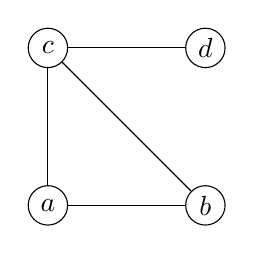
\begin{tikzpicture}[sommet/.style={draw, circle, inner sep=0pt, minimum size=5mm}]
    % Sommets
    \node[sommet] at (0,0) (a) {$a$};
    \node[sommet] at (2,0) (b) {$b$};
    \node[sommet] at (0,2) (c) {$c$};
    \node[sommet] at (2,2) (d) {$d$};
    % Arêtes
    \path (a) edge (b) edge (c);
    \path (c) edge (b) edge (d);
  \end{tikzpicture}
  \caption{Le graphe $G = (V,E)$, où $V = \{a,b,c,d\}$ et $E = \{\{a,b\}, \{a,c\}, \{b,c\}, \{c,d\}\}$.}\label{F:graphe}
\end{figure}

\begin{figure}
  \centering
  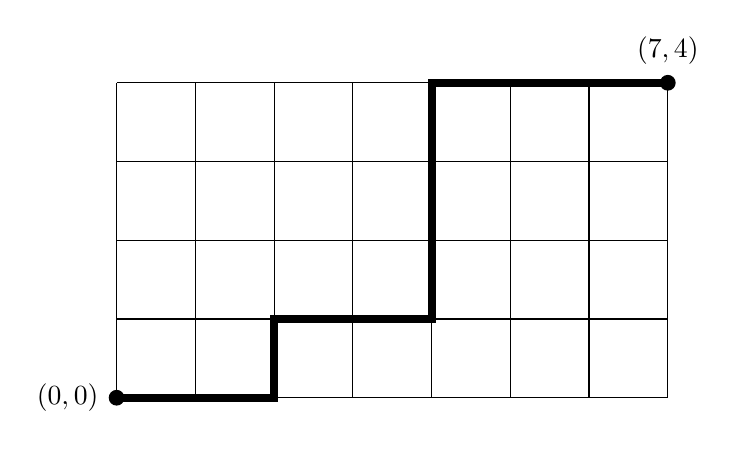
\begin{tikzpicture}[sommet/.style={fill=black, circle, inner sep=0pt, minimum size=2mm}]
    % Grille
    \draw (0,0) grid (7,4);
    % Sommets
    \node[sommet, label=180:{$(0,0)$}] at (0,0) (d) {};
    \node[sommet, label=90:{$(7,4)$}]  at (7,4) (f) {};
    % Chemin
    \draw[line width=1mm] (0,0) -- ++ (1,0) -- ++ (1,0) -- ++ (0,1) -- ++ (1,0) -- ++ (1,0) -- ++ (0,1) -- ++ (0,1) -- ++ (0,1) -- ++ (1,0) -- ++ (1,0) -- ++ (1,0);
  \end{tikzpicture}
  \caption{Une grille avec $r = 4$ et $c = 7$. Le chemin $ddhddhhhddd$ est représenté par un trait gras.}\label{F:grille}
\end{figure}

\end{document}
